\documentclass{beamer}
\usepackage{beamerthemeshadow}
\usepackage[utf8]{inputenc}
\usepackage[T1]{fontenc}
\usepackage{tikz}
\setbeamertemplate{navigation symbols}{}
\setbeamertemplate{section in toc}[sections numbered]
\setbeamertemplate{subsection in toc}[subsections numbered]
\setbeamertemplate{footline}[frame number]




%Information to be included in the title page:
\title{Potential energy surface of H$x$O$y$}
\author[Aribowo, Neumaier] % (optional, for multiple authors)
{Beryl Ramadhian Aribowo and Arnold Neumaier}

\institute[VFM] % (optional)
{
  Faculty of Mathematics\\
  University of Vienna
}
\date[VGSCO 2021] % (optional)
{VGSCO Seminar}



\begin{document}

\frame{\titlepage}

\begin{frame}
    \frametitle{Outline}
    \begin{columns}[t]
        \begin{column}{.6\textwidth}
            \tableofcontents[sections={1-2}]
        \end{column}
        \begin{column}{.4\textwidth}
            \tableofcontents[sections={3-5}]
        \end{column}
    \end{columns}
\end{frame}



\section{Introduction}
\subsection{Atoms \& molecules}
\begin{frame}{Atoms \& molecules}
    \begin{itemize}
        \item The \textbf{nuclear geometry}
    \end{itemize}
    \begin{figure}[htbp]
        \centering
        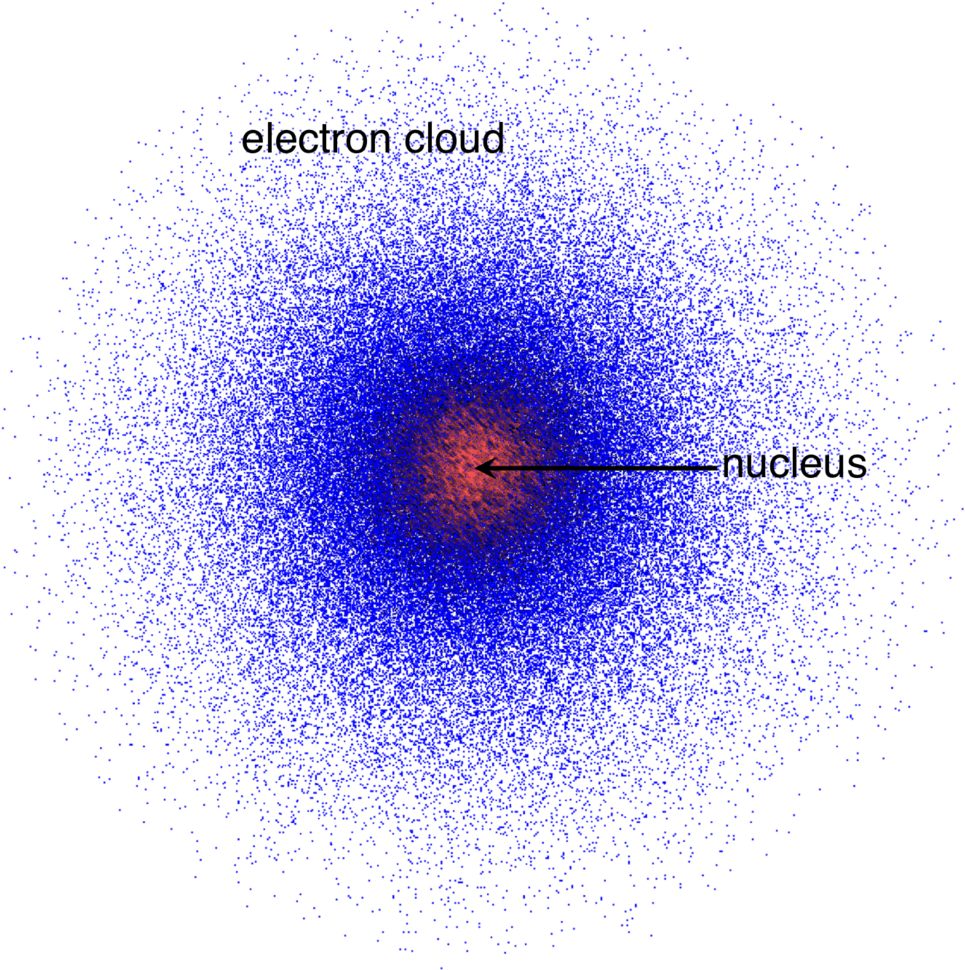
\includegraphics[scale=0.2]{img/slide/nuclear_geometry.png}
        \label{fig:nucleargeometry}
    \end{figure}
\end{frame}


\begin{frame}{Atoms \& molecules}
    \begin{itemize}
        \item The \textbf{molecular structure}
        \begin{figure}[htbp]
            \centering
            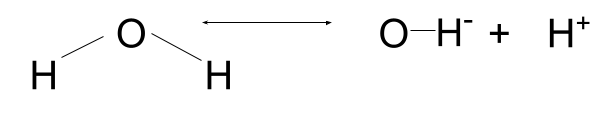
\includegraphics[scale=0.3]{img/slide/atoms_molecules.png}
            \label{fig:h2o}
        \end{figure}
    \end{itemize}
\end{frame}

\begin{frame}{Atoms \& molecules}
    ins somethng
\end{frame}

\subsection{Spectroscopic notation \& energy level}
\begin{frame}{Spectroscopic notation \& energy level}
    \begin{itemize}
        \item Example: H$_2(X^1\Sigma_g^+)$
    \end{itemize}
\end{frame}

\subsection{Potential energy surface (PES)}
\begin{frame}{PES}
    PES is
\end{frame}
\subsection{Applications}
\subsection{Short history of PES}
\subsection{Research framework}
\section{Related works}
\subsection{Permutation symmetry}
\subsection{Local PES}
\subsection{Global PES}
\subsection{Pair potentials}
\section{Results}
\subsection{Pair potential ansatz}
\subsection{Data aspects}
\subsection{Computational results}
\section{Future works}
\subsection{Multivalued fit}
\subsection{Many-body potential}
\subsection{Finding conical intersection}
\subsection{Potential for H$x$O$y$}
\section{References}

\begin{frame}\frametitle{Title} 
Each frame should have a title.
\end{frame}

\begin{frame} 
Without title somethink is missing. 
\begin{table}[h]
\caption{Atomic energy conversion factors.}
\begin{tabular}{|c|c|c|c|c|c|}
\hline
                   & \textbf{Hartree}         & \textbf{eV}              & \textbf{kcal/mol} & \textbf{kJ/mol} & \textbf{cm$^{-1}$} \\ \hline
\textbf{Hartree}   & 1                        & 27.2107                  & 627.503           & 2625.5          & 219474.63          \\ \hline
\textbf{eV}        & 0.0367502                & 1                        & 23.0609           & 96.486 9        & 8065.73            \\ \hline
\textbf{kcal/mol}  & 0.00159362               & 0.0433634                & 1                 & 4.18400         & 349.757            \\ \hline
\textbf{kJ/mol}    & 0.00038088               & 0.01036410               & 0.239001          & 1               & 83.593             \\ \hline
\textbf{cm$^{-1}$} & $4.55633 \times 10^{-6}$ & $1.23981 \times 10^{-4}$ & 0.00285911        & 0.0119627       & 1                  \\ \hline
\end{tabular}
\label{tb:dataunitconv}
\end{table}

\end{frame}




\end{document}